Cette annexe présente le code source des scripts Matlab implémentant les
concepts présentés dans cet ouvrage, soit l'arrimage de blocs, la mesure des
effets de bloc compensés par le mouvement et la distribution de bordures. Au
besoin, un diagramme de classe UML est utilisé pour présenter les scripts
associés à un sujet et les liens entre ceux-ci.

\begin{section}{L'arrimage de blocs \ang{Block Matching}}
L'arrimage de blocs se fait dans le script \textit{blockMatching.m}. Cependant,
afin de découpler ce script à l'algorithme de recherche de bloc candidat
(\textit{fullSearch.m}) ainsi qu'à l'évaluation de la corrélation entre les
blocs (\textit{SAD.m}), ses notions ont été développées dans des scripts à part,
interchangeable.

\begin{figure}
	\fbox{ % cette commande est nécéssaire pour encadrer les figures
	\centering
		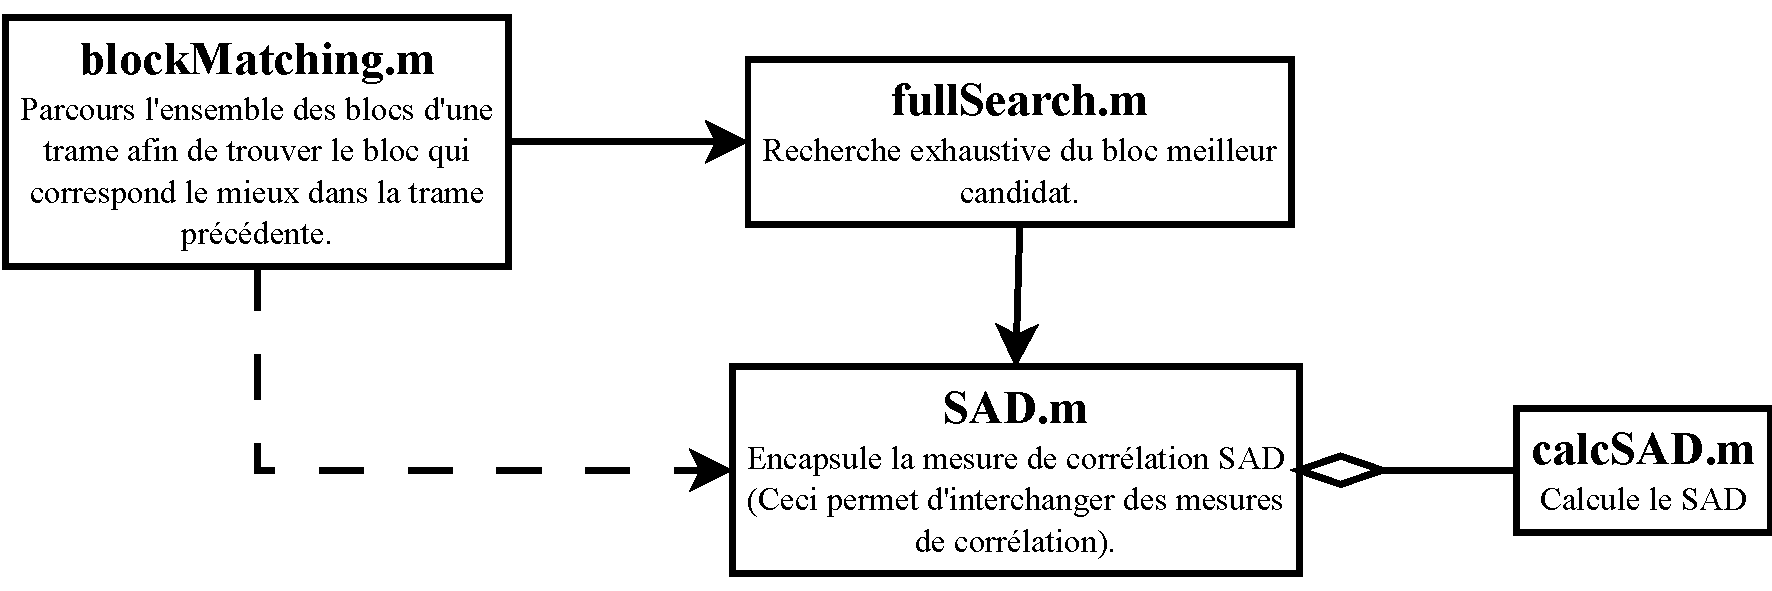
\includegraphics[width=0.97\linewidth]{Annexe/matlab/ArrimageBlocs.pdf} }
	\caption{Diagramme UML de classes des fichiers script utilisés pour l'arrimage
	de blocs.}
	\label{fig-BlockMatchingUML}
\end{figure}

\newpage

\lstinputlisting[caption=blockMatching.m]{Annexe/matlab/blockMatching.m}
\newpage
\lstinputlisting[caption=fullSearch.m]{Annexe/matlab/fullSearch.m}
\lstinputlisting[caption=SAD.m]{Annexe/matlab/SAD.m}
\lstinputlisting[caption=calcSAD.m]{Annexe/matlab/calcSAD.m}
\FloatBarrier
\end{section}

\begin{section}{Évaluation des effets de blocs compensés par le mouvement
(MCB).} À l'aide des vecteurs de mouvement issus de l'arrimage de blocs de la
section précédente, nous sommes en mesure de calculer les effets de blocs
compensés par le mouvement (\textit{temporalBlockiness.m}). Notons que l'ancien
nom du \textit{motion compensated blockiness} était \textit{temporalBlockiness},
ce qui explique les noms de fichiers. Le script \textit{interpolateClasses.m}
n'est pas requis, mais permet de mesurer le MCB au demi-pixel.
\begin{figure}
	\fbox{ % cette commande est nécéssaire pour encadrer les figures
	\centering
		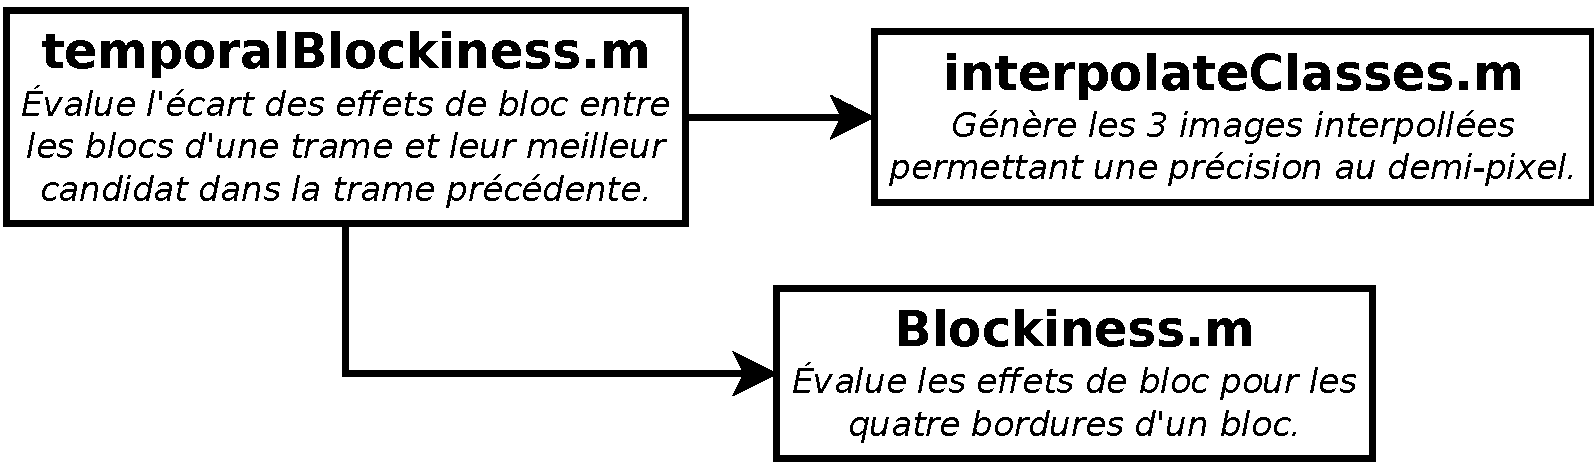
\includegraphics[width=0.97\linewidth]{Annexe/matlab/MCB.pdf} }
	\caption{Diagramme UML de classes des fichiers script utilisés pour mesurer
	les effets de bloc compensés par le mouvement.}
	\label{fig-BlockMatchingUML}
\end{figure}
\FloatBarrier

\newpage

\lstinputlisting[caption=temporalBlockiness.m]{Annexe/matlab/temporalBlockiness.m}
\lstinputlisting[caption=interpolateClasses.m]{Annexe/matlab/interpolateClasses.m}
\newpage
\lstinputlisting[caption=blockiness.m]{Annexe/matlab/blockiness.m}
\end{section}

\newpage

\begin{section}{Distribution de bordures}
Finalement, la distribution des bordures issue du MCB est accomplie à l'aide du
script \textit{enhanceBlockiness.m}.
\lstinputlisting[caption=enhanceBlockiness.m]{Annexe/matlab/enhanceBlockiness.m}
\end{section}